% =====================================================================
% SOUTENANCE DE MASTER — KENFACK Leonel — ORACLE
% Presentation Beamer, ~40 diapositives, un message par diapositive.
% Fil conducteur = structure du memoire (My-Thesis.tex).
% Compilation :  cd memoire && pdflatex soutenance.tex  (x2)
% =====================================================================
\documentclass[aspectratio=169,10pt]{beamer}

\usepackage[utf8]{inputenc}
\usepackage[T1]{fontenc}
\usepackage[french]{babel}
\usepackage{lmodern}
\usepackage{amsmath, amssymb}
\usepackage{booktabs}
\usepackage{tikz}
\usetikzlibrary{positioning, fit, arrows.meta, calc}

% ------------------- Couleurs URIFIA (identiques au memoire) --------
\definecolor{uridarkblue}{RGB}{30,40,90}
\definecolor{urigray}{RGB}{70,70,70}
\definecolor{uriaccent}{RGB}{180,60,40}

% ------------------- Macros du memoire -------------------------------
\newcommand{\Oracle}{\textsc{Oracle}}
\newcommand{\CorrDiff}{\textsc{CorrDiff}}
\newcommand{\LR}{\mathrm{LR}}
\newcommand{\HR}{\mathrm{HR}}
\newcommand{\muHR}{\mu_{\HR}}
\newcommand{\Adag}{A_{\mathrm{dag}}}
\newcommand{\xHR}{x_{\HR}}
\newcommand{\yLR}{y_{\LR}}
\newcommand{\HT}{H_T}

% ------------------- Theme minimal ----------------------------------
\usetheme{default}
\setbeamertemplate{navigation symbols}{}
\setbeamersize{text margin left=0.9cm, text margin right=0.9cm}

\setbeamercolor{structure}{fg=uridarkblue}
\setbeamercolor{frametitle}{fg=uridarkblue, bg=white}
\setbeamercolor{title}{fg=uridarkblue}
\setbeamercolor{normal text}{fg=black!85}
\setbeamercolor{alerted text}{fg=uriaccent}
\setbeamercolor{block title}{fg=white, bg=uridarkblue}
\setbeamercolor{block body}{fg=black!85, bg=uridarkblue!6}
\setbeamercolor{block title alerted}{fg=white, bg=uriaccent}
\setbeamercolor{block body alerted}{fg=black!85, bg=uriaccent!6}
\setbeamercolor{block title example}{fg=white, bg=green!40!black}
\setbeamercolor{block body example}{fg=black!85, bg=green!40!black!6}
\setbeamercolor{section in toc}{fg=uridarkblue}
\setbeamercolor{footline}{fg=white, bg=uridarkblue}

\setbeamerfont{frametitle}{series=\bfseries, size=\large}
\setbeamerfont{title}{series=\bfseries, size=\Large}
\setbeamerfont{footline}{size=\tiny}

\setbeamertemplate{frametitle}{%
  \vspace*{0.35cm}%
  \insertframetitle\par
  \vspace*{0.05cm}%
  {\color{uriaccent}\rule{1.6cm}{1.2pt}}\par
  \vspace*{-0.1cm}%
}

\setbeamertemplate{itemize item}{\color{uriaccent}\scriptsize$\blacktriangleright$}
\setbeamertemplate{itemize subitem}{\color{uridarkblue}\scriptsize$\bullet$}

\setbeamertemplate{footline}{%
  \begin{beamercolorbox}[wd=\paperwidth, ht=2.4ex, dp=1.1ex]{footline}%
    \hspace*{0.9cm}%
    KENFACK Leonel%
    \hfill Soutenance de Master --- \Oracle{}%
    \hfill \insertsectionhead%
    \hfill \insertframenumber\,/\,\inserttotalframenumber%
    \hspace*{0.9cm}%
  \end{beamercolorbox}%
}

% Table style helper
\newcommand{\tgood}[1]{\textcolor{green!40!black}{\textbf{#1}}}
\newcommand{\tbad}[1]{\textcolor{uriaccent}{#1}}

\begin{document}

% =====================================================================
% 1 — TITRE
% =====================================================================
\begin{frame}[plain]
  \begin{columns}[c]
    \begin{column}{0.30\textwidth}
      \centering\footnotesize
      \textbf{RÉPUBLIQUE DU CAMEROUN}\\
      \emph{Paix -- Travail -- Patrie}\\[2pt]
      \textbf{UNIVERSITÉ DE DSCHANG}\\
      École des Sciences et\\ Technologies de Dschang
    \end{column}
    \begin{column}{0.30\textwidth}
      \centering
      
\includegraphics[width=2.1cm]{My-Thesis/images/logouniv.png}
    \end{column}
    \begin{column}{0.30\textwidth}
      \centering\footnotesize
      \textbf{REPUBLIC OF CAMEROON}\\
      \emph{Peace -- Work -- Fatherland}\\[2pt]
      \textbf{UNIVERSITY OF DSCHANG}\\
      School of Sciences and\\ Technologies of Dschang
    \end{column}
  \end{columns}

  \vspace{0.5cm}
  \centering
  {\footnotesize Unité de Recherche en Informatique Fondamentale, Ingénierie et Applications (URIFIA)}\\[0.35cm]
  \begin{tikzpicture}
    \node[draw=uridarkblue!75, line width=0.7pt, rounded corners=8pt,
          inner sep=10pt, text width=0.8\linewidth, align=center,
          top color=uridarkblue!16, bottom color=teal!10] {%
      \color{uridarkblue}\large\bfseries
      Développement de Méthodes d'Apprentissage Automatique pour la\\
      Mise à l'Échelle Spatiale des Données Climatiques};
  \end{tikzpicture}\\[0.35cm]
  {\small Mémoire de Master en Informatique --- option Informatique Fondamentale, spécialisation Intelligence Artificielle}\\[0.3cm]
  {\normalsize Présenté par \textbf{\textcolor{uridarkblue}{KENFACK Leonel}}}\\[0.1cm]
  {\small Sous la direction du \textbf{Pr.~BOMGNI Alain Bertrand}, Maître de Conférences}\\[0.3cm]
  {\footnotesize\itshape Année académique 2025--2026}
\end{frame}

% =====================================================================
% 2 — PLAN
% =====================================================================
\begin{frame}{Plan de l'exposé}
  \vspace{0.2cm}
  \begin{columns}[T]
    \begin{column}{0.55\textwidth}
      \tableofcontents
    \end{column}
    \begin{column}{0.41\textwidth}
      \begin{block}{Le fil de l'exposé}
        \small
        Un besoin local vital $\to$ un verrou scientifique précis $\to$
        une réponse architecturale, \Oracle{} $\to$ des résultats mesurés
        contre une baseline stricte $\to$ des limites assumées.
      \end{block}
    \end{column}
  \end{columns}
\end{frame}

% =====================================================================
\section{Contexte et problématique}
% =====================================================================

% 3 — C'EST QUOI LE DOWNSCALING
\begin{frame}{Les modèles climatiques globaux voient le monde à 100--250 km}
  \begin{columns}[c]
    \begin{column}{0.56\textwidth}
      \begin{itemize}
        \item Les GCM du GIEC (CMIP6) simulent l'atmosphère avec des mailles
              de \alert{100 à 250 km} de côté.
        \item À cette échelle : Douala et Yaoundé occupent \alert{la même cellule},
              le mont Cameroun n'a aucun effet, la transition savane--forêt disparaît.
        \item \textbf{Downscaling} (descente d'échelle) : produire, à partir de ces
              sorties grossières, une représentation fine (\alert{1 à 12 km})
              utilisable pour la décision.
      \end{itemize}
    \end{column}
    \begin{column}{0.40\textwidth}
      \centering
      \begin{tikzpicture}[scale=0.9]
        % grille grossiere
        \draw[step=1.0, urigray!70, thick] (0,0) grid (2,2);
        \node[font=\scriptsize, text=urigray] at (1,-0.35) {GCM : $\sim$150 km};
        % fleche
        \draw[-{Stealth[length=3mm]}, very thick, uriaccent] (2.4,1) -- (3.4,1)
          node[midway, above, font=\scriptsize\bfseries, text=uriaccent] {$\times 25$};
        % grille fine
        \draw[step=0.2, uridarkblue!60] (3.8,0) grid (5.8,2);
        \draw[uridarkblue, thick] (3.8,0) rectangle (5.8,2);
        \node[font=\scriptsize, text=uridarkblue] at (4.8,-0.35) {Cible : 5--10 km};
      \end{tikzpicture}

      \vspace{0.3cm}
      {\footnotesize Même territoire, deux lectures : \\ l'une invisible aux décideurs, l'autre exploitable.}
    \end{column}
  \end{columns}
\end{frame}

% 4 — POURQUOI
\begin{frame}{Pourquoi ? Les décisions d'adaptation se prennent à l'échelle locale}
  \begin{itemize}
    \item \textbf{Agriculture} : semer quoi, où, quand --- la planification d'un bassin
          agricole pluvial dépend de la pluie \emph{locale}, pas de la moyenne régionale.
    \item \textbf{Eau et énergie} : dimensionner un barrage ou un réseau de drainage
          exige la distribution fine des précipitations, extrêmes compris.
    \item \textbf{Urbanisme et risque} : les inondations de l'Extrême-Nord du Cameroun
          (octobre 2024) ont affecté \alert{356\,000 personnes} et noyé
          \alert{82\,500 hectares} de cultures --- \emph{sans qu'aucune anticipation
          communale n'ait été possible}.
  \end{itemize}
  \vspace{0.2cm}
  \begin{alertblock}{Le message}
    Sans downscaling, les projections climatiques existent mais restent
    \emph{inutilisables} là où elles seraient le plus nécessaires.
  \end{alertblock}
\end{frame}

% 5 — INTERET EN AFRIQUE
\begin{frame}{En Afrique, le besoin est vital et les moyens de calcul manquent}
  \begin{columns}[T]
    \begin{column}{0.48\textwidth}
      \textbf{Le besoin}
      \begin{itemize}
        \item Cameroun : l'agriculture pèse \alert{22\,\% du PIB} et fait vivre
              \alert{44\,\%} de la population active (Banque Mondiale).
        \item La centrale de Lagdo fournit \alert{74\,\%} de l'électricité du Nord-Cameroun.
        \item Productivité agricole africaine : \alert{$-34\,\%$ depuis 1961} sous l'effet
              du changement climatique (GIEC AR6), pire régression mondiale.
        \item Sans adaptation : \alert{4 à 10\,\% du PIB} camerounais menacé d'ici 2050.
      \end{itemize}
    \end{column}
    \begin{column}{0.48\textwidth}
      \textbf{Les moyens}
      \begin{itemize}
        \item Le continent héberge \alert{moins de 1\,\%} des capacités mondiales
              de calcul haute performance.
        \item Le downscaling dynamique classique y est donc \emph{de facto} hors
              de portée en production locale.
      \end{itemize}
      \vspace{0.2cm}
      \begin{block}{Conséquence}
        \small Il faut des méthodes de downscaling \emph{peu coûteuses à l'inférence}
        et \emph{fiables hors de leur régime d'entraînement}.
      \end{block}
    \end{column}
  \end{columns}
\end{frame}

% 6 — DEUX FAMILLES
\begin{frame}{Deux familles de downscaling, deux impasses différentes}
  \begin{columns}[T]
    \begin{column}{0.48\textwidth}
      \begin{block}{Dynamique (RCM emboîté)}
        \small
        \begin{itemize}
          \item Résout les équations physiques à maille fine : \tgood{rigoureux}.
          \item Mais la configuration CWA-WRF de référence tourne sur
                \alert{928 c\oe{}urs en parallèle} : un seul scénario à la fois,
                résolutions CORDEX bloquées à 12--50 km.
        \end{itemize}
      \end{block}
    \end{column}
    \begin{column}{0.48\textwidth}
      \begin{block}{Statistique (apprentissage profond)}
        \small
        \begin{itemize}
          \item Apprend $\yLR \mapsto \xHR$ : \tgood{rapide}, milliers de membres possibles.
          \item Mais \emph{boîte noire} : sorties impossibles ($T_{\min}>T_{\max}$,
                4\,\% $\to$ 15--17\,\% en projection 2100), 31 réentraînements identiques
                $\Rightarrow$ erreurs variant d'un \alert{facteur 46}.
        \end{itemize}
      \end{block}
    \end{column}
  \end{columns}
  \vspace{0.25cm}
  \centering
  \small Ce mémoire s'inscrit dans la seconde voie --- \alert{en s'attaquant à ses défauts
  d'interprétabilité et de généralisation}.
\end{frame}

% 7 — TROIS VERROUS
\begin{frame}{La littérature fait ressortir trois verrous structurants}
  \begin{enumerate}
    \item \textbf{Stabilité d'entraînement.} Les GAN sont très sensibles au poids
          adversarial $\lambda_{\mathrm{adv}}$ et au déséquilibre générateur--discriminateur ;
          réglages peu transférables d'une région à l'autre.
    \item \textbf{Réalisme des extrêmes (sub-dispersion).} Variance prédite trop faible :
          $\sigma_{\mathrm{pred}}/\mathrm{RMSE} \approx \alert{0{,}3}$ rapporté dans le domaine
          (cible : $1$), soit un facteur 3 de sous-estimation de la variabilité ---
          donc des extrêmes, précisément les événements à plus forte valeur.
    \item \textbf{Robustesse hors-distribution.} Sous changement climatique, la statistique
          jointe des variables évolue ; un modèle purement corrélatif apprend des
          associations contingentes au régime d'entraînement.
  \end{enumerate}
\end{frame}

% 8 — TRILEMME
\begin{frame}{Aucune approche ne tient les trois sommets à la fois : un trilemme}
  \begin{columns}[c]
    \begin{column}{0.52\textwidth}
      \centering
      \resizebox{0.92\linewidth}{!}{%
      \begin{tikzpicture}[scale=0.82,
        vertex/.style={font=\footnotesize\bfseries, text=uridarkblue, align=center},
        method/.style={circle, draw, thick, inner sep=2.5pt, font=\scriptsize},
        methodlbl/.style={font=\scriptsize\sffamily, align=center}]
        \coordinate (top)   at (0, 3.46);
        \coordinate (left)  at (-3, -1.5);
        \coordinate (right) at (3, -1.5);
        \draw[thick, uridarkblue] (top) -- (left) -- (right) -- cycle;
        \node[vertex, above=0.12cm of top] {Stabilité\\ d'entraînement};
        \node[vertex, below left=0.05cm and -0.5cm of left] {Réalisme\\ des extrêmes};
        \node[vertex, below right=0.05cm and -0.5cm of right] {Robustesse\\ OOD};
        \node[method, fill=red!25] (cgan) at (-1.6, -0.6) {};
        \node[methodlbl, below=2pt of cgan, text=red!60!black] {cGAN};
        \node[method, fill=orange!40] (corrdiff) at (0.7, 1.0) {};
        \node[methodlbl, above right=-2pt and 0pt of corrdiff, text=orange!70!black] {\CorrDiff};
        \node[method, fill=uriaccent!70] (oracle) at (0.4, 0.05) {};
        \node[methodlbl, right=2pt of oracle, text=uriaccent] {\Oracle};
        \node[method, fill=green!55!black] (ideal) at (-0.35, 0.15) {};
        \node[methodlbl, below=2pt of ideal, text=green!45!black] {Idéal};
      \end{tikzpicture}%
      }
    \end{column}
    \begin{column}{0.44\textwidth}
      \small
      \begin{itemize}
        \item Les cGAN les plus \textbf{expressifs} sont les plus \tbad{instables}.
        \item Les diffusions \textbf{stables} restent \tbad{corrélatives}, sans garantie OOD.
        \item Les RCM \textbf{robustes} paient en \tbad{coût de calcul}.
      \end{itemize}
      \vspace{0.2cm}
      {\footnotesize Constat agrégé de la littérature (Rampal 2024, Mardani 2023,
      Harris 2022) --- pas une formalisation originale.}
    \end{column}
  \end{columns}
\end{frame}

% 9 — PROBLEMATIQUE
\begin{frame}{Problématique}
  \vspace{0.4cm}
  \begin{block}{La question centrale du mémoire}
    \centering
    \emph{Comment \alert{causaliser le premier étage} du paradigme à deux étages
    pour doter le downscaling probabiliste d'une \alert{robustesse de principe}
    au changement de distribution, \alert{sans dégrader} la stabilité ni le
    réalisme acquis ?}
  \end{block}
  \vspace{0.35cm}
  \small Trois termes à défendre aujourd'hui :
  \begin{itemize}
    \item \textbf{causaliser} : quelle forme de causalité, placée où ? (Proposition)
    \item \textbf{robustesse de principe} : comment la mesurer honnêtement ? (Protocole)
    \item \textbf{sans dégrader} : contre quelle référence ? (Baseline stricte)
  \end{itemize}
\end{frame}

% =====================================================================
\section{État de l'art}
% =====================================================================

% 10 — cGAN
\begin{frame}{Les cGAN résiduels : nets sur les extrêmes, fragiles à l'entraînement}
  \begin{itemize}
    \item Référence du domaine néo-zélandais : le cGAN résiduel de Rampal et al.\ (2024) ---
          un CNN prédit la moyenne, un générateur adversarial ajoute les détails.
    \item \tgood{Forces} : champs nets, bonne texture des fortes pluies, inférence rapide.
    \item \tbad{Limites empiriques} : instabilité générateur--discriminateur,
          \emph{mode collapse}, pas de vraisemblance explicite --- et sub-dispersion
          persistante.
  \end{itemize}
  \vspace{0.2cm}
  \begin{block}{Ce qu'on en retient pour \Oracle{}}
    \small L'idée \emph{résiduelle} (prédire l'écart à une moyenne) est précieuse ;
    le cadre adversarial, lui, compromet le verrou n°1 (stabilité).
  \end{block}
\end{frame}

% 11 — DIFFUSION EDM
\begin{frame}{Les modèles de diffusion : le cadre stable, formalisé par EDM}
  \begin{itemize}
    \item Principe : apprendre à débruiter progressivement un champ, puis échantillonner
          en partant du bruit --- entraînement par simple régression, \tgood{stable}.
    \item Le formalisme EDM (Karras et al., 2022) \textbf{normalise adaptativement}
          entrées et sorties selon le niveau de bruit $\sigma$ :
  \end{itemize}
  \begin{equation*}
    \mathcal{D}_\theta(x_\sigma, \sigma) = c_{\mathrm{skip}}(\sigma)\, x_\sigma
      + c_{\mathrm{out}}(\sigma)\, \epsilon_\theta\!\big( c_{\mathrm{in}}(\sigma)\, x_\sigma,\; c_{\mathrm{noise}}(\sigma) \big)
  \end{equation*}
  \begin{itemize}
    \item Le réseau reçoit un signal d'apprentissage stable sur toute la plage de bruit :
          plus d'hyperparamètres de schéma à régler à la main.
    \item \tbad{Mais} : un modèle de diffusion reste \emph{corrélatif} --- rien ne
          contraint ce qu'il apprend à survivre à un changement de régime.
  \end{itemize}
\end{frame}

% 12 — CORRDIFF
\begin{frame}{\CorrDiff{} : régression déterministe puis diffusion du résidu}
  \begin{columns}[c]
    \begin{column}{0.52\textwidth}
      \centering
      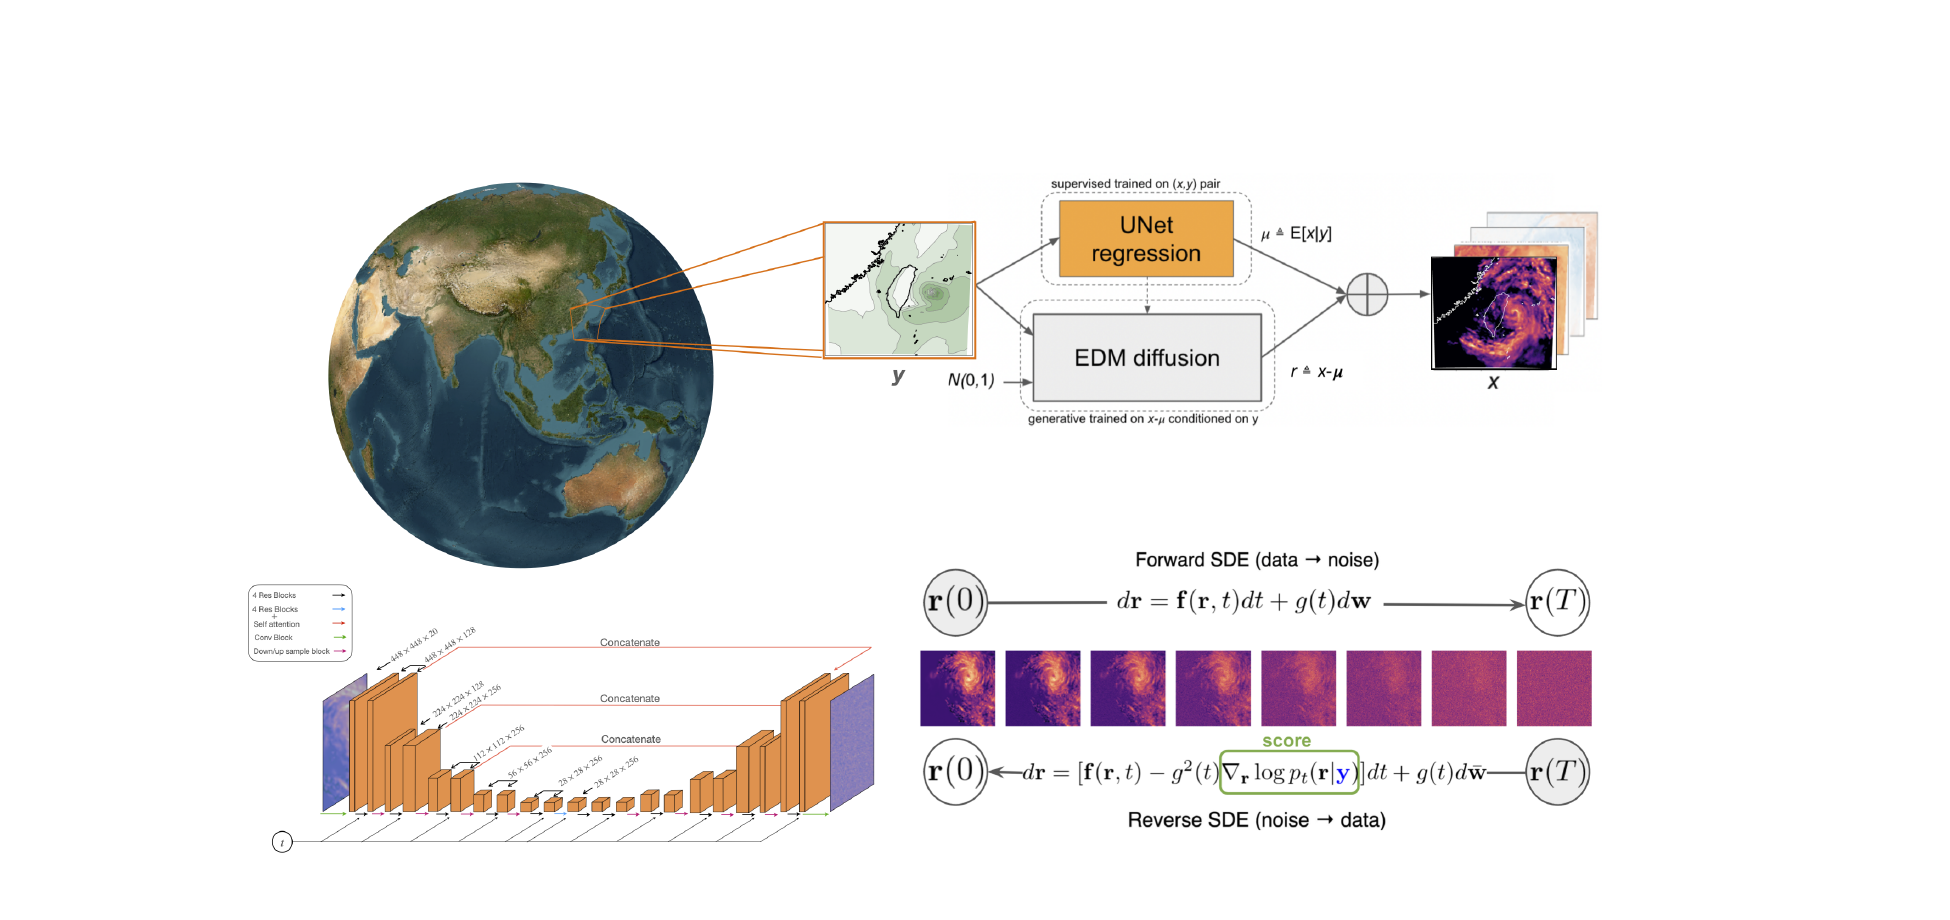
\includegraphics[width=\linewidth]{../results/literature_figures/mardani_corrdiff_fig1.png}
      \par{\scriptsize Figure : Mardani et al.\ (2023), reproduite au chapitre I du mémoire.}
    \end{column}
    \begin{column}{0.44\textwidth}
      \small
      \begin{itemize}
        \item \textbf{Étage 1} : un U-Net entraîné par MSE prédit la moyenne conditionnelle.
        \item \textbf{Étage 2} : une diffusion EDM échantillonne le \emph{résidu} ---
              cible centrée, de faible amplitude.
        \item Résultat : $\sim$\alert{$60\times$} la vitesse d'un RCM WRF à l'inférence,
              calibration correcte.
      \end{itemize}
      \vspace{0.15cm}
      {\footnotesize C'est le paradigme que nous adoptons --- et que nous allons
      modifier en un point précis.}
    \end{column}
  \end{columns}
\end{frame}

% 13 — LIMITES CORRDIFF
\begin{frame}{Deux failles de \CorrDiff{} : stationnarité supposée, conditionnement contournable}
  \begin{enumerate}
    \item \textbf{Hypothèse de stationnarité.} L'efficacité du schéma résiduel repose sur la
          \emph{faible variance du résidu}, garantie seulement si la distribution cible est
          stationnaire --- hypothèse que le changement climatique invalide directement.
          Les auteurs signalent eux-mêmes un \emph{significant distribution shift}.
    \item \textbf{Le piège du conditionnement par cross-attention.} Une voie d'attention
          parallèle permet au réseau de puiser l'information \emph{en contournant} le
          module que l'on croit conditionnant.
  \end{enumerate}
  \vspace{0.2cm}
  \begin{alertblock}{Constat vécu (phases exploratoires 1--2 du projet)}
    \small Avec un conditionnement par cross-attention, notre DAG appris était
    \emph{décoratif} : forcer $\Adag \leftarrow \mathbf{0}$ ne dégradait pas la
    prédiction. Le U-Net bypassait le chemin causal via ses skip-connections.
  \end{alertblock}
\end{frame}

% 14 — TABLEAU / GAP
\begin{frame}{Le gap : aucune approche n'intègre de structure causale par construction}
  \centering
  \small
  \begin{tabular}{l c c c c c}
    \toprule
    \textbf{Approche} & \textbf{Stabilité} & \textbf{Extrêmes} & \textbf{OOD} & \textbf{Causal} & \textbf{Génératif} \\
    \midrule
    U-Net / CNN (2017)        & \checkmark & $\times$    & $\times$    & $\times$   & $\times$   \\
    cGAN résiduel (2024)      & $\triangle$ & $\triangle$ & $\times$    & $\times$   & \checkmark \\
    DDPM / EDM brut (2020-22) & \checkmark & \checkmark  & $\triangle$ & $\times$   & \checkmark \\
    \CorrDiff{} (2023)        & \checkmark & $\triangle$ & $\triangle$ & $\times$   & \checkmark \\
    \midrule
    \textbf{\Oracle{} (proposé)} & \checkmark & $\triangle$ & $\triangle$ & \tgood{\checkmark} & \checkmark \\
    \bottomrule
  \end{tabular}
  \par\vspace{0.15cm}
  {\scriptsize \checkmark{} = bien traité \quad $\triangle$ = partiel \quad $\times$ = non
  traité. Extrait du tableau modèle$\times$verrou du chapitre II ; les $\triangle$
  d'\Oracle{} reflètent honnêtement les limites mesurées.}
  \vspace{0.2cm}
  \begin{block}{Formulation du gap}
    \small Le paradigme deux-étages couvre le mieux stabilité $+$ extrêmes $+$ probabiliste,
    mais sa robustesse OOD n'est pas adressée \emph{par construction} :
    il faut \alert{causaliser son premier étage}.
  \end{block}
\end{frame}

% =====================================================================
\section{Proposition : \Oracle{}}
% =====================================================================

% 15 — OBJECTIFS
\begin{frame}{Ce que nous proposons}
  \textbf{Objectif principal.} Une architecture de downscaling probabiliste intégrant une
  structure causale \emph{apprise}, qui garantit \emph{par construction} la dépendance
  entre variables atmosphériques d'entrée et précipitation prédite.
  \vspace{0.25cm}
  \begin{enumerate}
    \item Concevoir un \textbf{réseau causal récurrent} (RCN) : SCM dynamique $+$ GRU $+$
          pénalité d'acyclicité DAGMA, dans une seule cellule ;
    \item L'inscrire dans le paradigme deux-étages de \CorrDiff{} en remplaçant
          \emph{uniquement} le premier étage --- l'étage de diffusion EDM reste
          \alert{inchangé} ;
    \item Définir un \textbf{protocole} centré sur la calibration probabiliste, le réalisme
          des extrêmes et la robustesse inter-GCM, incluant un test d'intervention
          contrôlée original dans ce contexte.
  \end{enumerate}
\end{frame}

% 16 — IDEE CLE
\begin{frame}{L'idée clé : placer la causalité dans la topologie, pas dans la perte}
  \begin{columns}[T]
    \begin{column}{0.48\textwidth}
      \begin{alertblock}{Causalité par régularisation}
        \small Un terme de perte « causal » peut être \alert{contourné} par un réseau
        suffisamment expressif : il minimise la pénalité sans changer son mécanisme.
      \end{alertblock}
    \end{column}
    \begin{column}{0.48\textwidth}
      \begin{exampleblock}{Causalité par architecture}
        \small Une dépendance inscrite dans le \emph{graphe de calcul} est
        \alert{indéfaisable par construction} : aucune information conditionnelle
        ne peut transiter ailleurs que par $\Adag$.
      \end{exampleblock}
    \end{column}
  \end{columns}
  \vspace{0.35cm}
  \centering
  \small C'est un déplacement du \emph{lieu} de la contrainte : de la fonction objectif
  vers la topologie du réseau. Toute la conception d'\Oracle{} découle de ce choix ---
  et il se \textbf{teste} (propriété O3, plus loin).
\end{frame}

% 17 — VUE D'ENSEMBLE
\begin{frame}{\Oracle{} en quatre blocs, autour d'une décomposition additive}
  \begin{equation*}
    \xHR \;=\; \underbrace{\mathrm{baseline}_{\LR\uparrow}}_{\text{interpolation}}
    \;+\; \underbrace{\muHR\!\left(\yLR;\, \Adag\right)}_{\text{moyenne causale (Étage 1)}}
    \;+\; \underbrace{\delta\!\left(\sigma;\, \muHR, \mathrm{baseline}\right)}_{\text{résidu stochastique (Étage 2)}}
  \end{equation*}
  \centering
  \resizebox{0.96\linewidth}{!}{%
  \begin{tikzpicture}[
      blk/.style={rectangle, draw=uridarkblue, fill=uridarkblue!10, rounded corners,
                  minimum height=0.95cm, minimum width=1.9cm, align=center, font=\footnotesize},
      cblk/.style={rectangle, draw=uriaccent, fill=uriaccent!10, rounded corners,
                  minimum height=0.95cm, minimum width=1.9cm, align=center, font=\footnotesize},
      arr/.style={-{Stealth[length=2.2mm]}, thick, urigray}]
    \node[blk] (lr) {$\yLR$\\ \scriptsize 15 var $\times$ 3 niveaux};
    \node[blk, right=0.7cm of lr] (base) {(1) Baseline\\ \scriptsize bilinéaire};
    \node[cblk, right=0.7cm of base] (crm) {(2) Module causal\\ \scriptsize graphe + RCN $\to \muHR$};
    \node[blk, right=0.7cm of crm] (edm) {(3) Diffusion EDM\\ \scriptsize résidu $\delta$};
    \node[blk, right=0.7cm of edm] (sum) {(4) Somme\\ $\xHR$};
    \draw[arr] (lr) -- (base);
    \draw[arr] (base) -- (crm);
    \draw[arr] (crm) -- (edm);
    \draw[arr] (edm) -- (sum);
    \draw[arr] (base.south) to[out=-25, in=-155] (sum.south);
    \draw[arr, uriaccent] (crm.north) to[out=25, in=155] (sum.north);
  \end{tikzpicture}%
  }
  \par\vspace{0.15cm}
  \begin{block}{Attribution propre}
    \small L'écart avec \CorrDiff{} est \alert{entièrement concentré dans le bloc (2)} :
    Étage 2, pertes EDM, sampler et préconditionnement sont hérités tels quels.
    Toute amélioration mesurée est attribuable à la causalisation.
  \end{block}
\end{frame}

% 18 — GRAPHE HETEROGENE
\begin{frame}{Un graphe atmosphérique hétérogène, agrégé à 6 n\oe{}uds pour rester lisible}
  \begin{columns}[c]
    \begin{column}{0.55\textwidth}
      \small
      \begin{itemize}
        \item N\oe{}uds \textbf{GP850, GP500, GP250} : variables dynamiques aux trois
              niveaux de pression ; n\oe{}ud \textbf{SP\_HR} : statiques haute résolution
              (orographie, masque terre/mer).
        \item Trois types d'arêtes $=$ trois mécanismes physiques :
              \textbf{spatiales} (advection), \textbf{verticales} (convection),
              \textbf{statiques$\to$pression} (influence orographique).
        \item Version résolue : $\sim$32\,600 n\oe{}uds. Version expérimentale :
              \alert{6 n\oe{}uds typés} $\Rightarrow$ $\Adag \in \mathbb{R}^{6\times 6}$
              inter-variables, \emph{interprétable par un humain}.
      \end{itemize}
    \end{column}
    \begin{column}{0.41\textwidth}
      \centering
      \begin{tikzpicture}[
        gp/.style={circle, draw=uridarkblue, fill=uridarkblue!12, minimum size=1.05cm, font=\scriptsize\bfseries},
        sp/.style={circle, draw=uriaccent, fill=uriaccent!12, minimum size=1.05cm, font=\scriptsize\bfseries},
        arr/.style={-{Stealth[length=2mm]}, thick, uridarkblue!80}]
        \node[gp] (g250) at (0,3.3) {GP$_{250}$};
        \node[gp] (g500) at (0,2.2) {GP$_{500}$};
        \node[gp] (g850) at (0,1.1) {GP$_{850}$};
        \node[sp] (sp)   at (0,0)   {SP$_{\HR}$};
        \draw[arr] (g250) -- (g500);
        \draw[arr] (g500) -- (g850);
        \draw[arr] (g850) -- (sp);
        \node[font=\scriptsize, text=urigray, align=left, right=0.5cm of g500]
          {cascade verticale :\\ couplage quasi-\\géostrophique\\ descendant\\ (prior initial,\\ librement apprenable)};
      \end{tikzpicture}
    \end{column}
  \end{columns}
\end{frame}

% 19 — ENCODEUR INTELLIGIBLE
\begin{frame}{Un encodeur intelligible : quinze MLP dédiés, zéro paramètre partagé}
  \begin{itemize}
    \item Un MLP \emph{par couple} (variable, niveau de pression) : $u, v, w, q, t$
          $\times$ \{850, 500, 250\}\,hPa $\to$ latent de dimension $d = 128$ chacun.
    \item Aucun poids partagé entre variables : chaque ligne et colonne de $\Adag$
          conserve une \alert{identité physique} lisible.
  \end{itemize}
  \vspace{0.2cm}
  \begin{block}{Pourquoi c'est important}
    \small Avec un encodeur mélangeant les canaux (convolution standard), l'arête
    « $q_{850} \to$ précipitation » ne voudrait plus rien dire : l'interprétabilité
    du DAG se joue \emph{avant} le DAG, dans l'encodeur.
  \end{block}
\end{frame}

% 20 — RCN
\begin{frame}{Le RCN : le modèle causal structurel \emph{est} le moteur récurrent}
  À chaque pas $t$, deux briques en boucle fermée ($T = 8$ pas) :
  \begin{columns}[T]
    \begin{column}{0.52\textwidth}
      \textbf{1. Assignation SCM} (\emph{plan de vol})
      \begin{equation*}
        \hat{H}_t^{(i)} = f_i\!\big( \Adag^{(i,:)} \odot H_{t-1},\; x_t,\; \varepsilon_t^{(i)} \big)
      \end{equation*}
      {\small chaque variable $i$ est prédite \emph{uniquement} depuis ses parents dans
      $\Adag$ --- un MLP structurel $f_i$ par variable.}
    \end{column}
    \begin{column}{0.44\textwidth}
      \textbf{2. Mise à jour GRU} (\emph{instruments})
      \begin{equation*}
        H_t = (1 - z_t) \odot \hat{H}_t + z_t \odot \tilde{H}_t
      \end{equation*}
      {\small fusion de la prédiction théorique et de l'observation courante
      (portes $z_t, r_t$ standard).}
    \end{column}
  \end{columns}
  \vspace{0.3cm}
  \begin{block}{L'originalité}
    \small La transition d'état $H_{t} \to H_{t+1}$ \alert{est} l'assignation causale ---
    le SCM n'est pas un post-traitement appliqué à un état caché produit par ailleurs.
  \end{block}
\end{frame}

% 21 — DAGMA
\begin{frame}{Apprendre un graphe acyclique par descente de gradient : DAGMA}
  Chercher un DAG est combinatoire (croissance super-exponentielle en $N$).
  DAGMA (Bello et al., 2022) rend l'acyclicité \emph{différentiable} :
  \begin{equation*}
    h_{\mathrm{DAGMA}}(A;\, s) \;=\; -\log \det\!\left( s\,I - A \odot A \right) + N \log s,
    \qquad s > N \max_{i,j} |A_{i,j}|
  \end{equation*}
  \begin{itemize}
    \item $h_{\mathrm{DAGMA}}(A) = 0 \iff A$ représente un DAG ;
          gradient via l'inverse de $sI - A\odot A$, coût d'une décomposition LU.
    \item Dans \Oracle{}, combinée à une sparsité $L_1$ pour une matrice
          \alert{creuse et auditable} :
          $\;\mathcal{L}_{\mathrm{dag}} = \lambda_{\mathrm{DAGMA}}\, h_{\mathrm{DAGMA}}(\Adag) + \lambda_{L_1} \|\Adag\|_1$.
    \item Warmup de 5 époques : la contrainte monte en puissance une fois les
          représentations stabilisées.
  \end{itemize}
\end{frame}

% 22 — DECODEUR
\begin{frame}{Du graphe à la grille : cross-attention intermédiaire puis raffinement}
  L'état final $\HT \in \mathbb{R}^{B \times N \times d}$ devient une carte
  $\muHR \in \mathbb{R}^{B \times 1 \times 172 \times 179}$ :
  \begin{equation*}
    \tilde{\mu}_p = \sum_{n=1}^{N} \alpha_{p,n} V_n,
    \qquad
    \alpha_{p,n} = \mathrm{softmax}_n\!\left( \langle Q_p, K_n \rangle / \sqrt{d} \right)
  \end{equation*}
  \begin{itemize}
    \item Requêtes sur une grille intermédiaire $43\times 45$ (attention directe à
          $172\times179$ : matrice $30\,788 \times N$ prohibitive ; coût réduit
          d'un facteur 16), puis sur-échantillonnage bilinéaire $+$ raffinement
          convolutif léger.
    \item \textbf{Garde-fou} : skip conditionnel
          $\muHR = \alpha(\yLR)\,\mu_{\mathrm{causal}} + (1-\alpha(\yLR))\,\mu_{\mathrm{direct}}$,
          avec porte apprise contrainte $\alpha \geq \alert{0{,}6}$ --- le modèle ne peut
          pas devenir un « non-causal déguisé ».
  \end{itemize}
\end{frame}

% 23 — O3
\begin{frame}{La propriété (O3) : l'indispensabilité du chemin causal est \emph{testable}}
  \begin{block}{Définition (indispensabilité causale, O3)}
    Soit $\Delta_{O3} = \mathrm{MSE}\!\big(\muHR(\mathbf{0})\big) - \mathrm{MSE}\!\big(\muHR(\Adag)\big)$
    le surcoût d'erreur quand $\Adag$ est forcée à zéro à l'inférence.
    \Oracle{} satisfait (O3) au seuil $\tau$ si
    \begin{equation*}
      \frac{\Delta_{O3}}{\mathrm{MSE}\!\big(\muHR(\Adag)\big)} \;\geq\; \tau,
      \qquad \tau \in [0{,}05,\; 0{,}10].
    \end{equation*}
  \end{block}
  \vspace{0.15cm}
  \begin{itemize}
    \item Opérationnalisée par une variante d'ablation qui force $\Adag = \mathbf{0}$
          \emph{à l'inférence seulement} : si le DAG était décoratif, rien ne bougerait.
    \item C'est le critère qui a \alert{disqualifié} nos architectures à cross-attention
          (phases 1--2) --- et qui sert de \textbf{porte d'entrée} au second étage.
  \end{itemize}
\end{frame}

% 24 — STAGE 2 EDM
\begin{frame}{Étage 2 : diffusion du résidu, conditionnée par concaténation --- jamais par attention}
  \begin{equation*}
    \mathrm{input}_{\mathrm{UNet}} = \mathrm{concat}\!\big( \delta_{\mathrm{bruit\acute{e}}},\; \muHR,\; \log(1+\mathrm{baseline}) \big) \in \mathbb{R}^{B\times 3\times H\times W}
  \end{equation*}
  \begin{itemize}
    \item La concaténation force le U-Net à \emph{voir} $\muHR$ comme un canal d'image
          traité localement --- \alert{aucune voie d'information parallèle} (leçon des
          phases 1--2) ; et elle coûte moins cher que l'attention.
    \item Le résidu est une cible \emph{facile} : centré autour de zéro, écart-type
          $\sigma_{\mathrm{data}}$ après log-transformation --- la calibration retrouve
          un sens physique et la sub-dispersion recule (verrou n°2).
    \item Formalisme EDM repris \textbf{sans modification} : préconditionnement
          $(c_{\mathrm{skip}}, c_{\mathrm{out}}, c_{\mathrm{in}}, c_{\mathrm{noise}})$,
          perte pondérée $\lambda(\sigma)$, solveur de Heun / DPM-Solver++.
  \end{itemize}
\end{frame}

% =====================================================================
\section{Matériels et méthodes}
% =====================================================================

% 25 — POURQUOI LA NZ
\begin{frame}{Terrain d'essai : la Nouvelle-Zélande, un bac à sable exigeant}
  Faute de jeu haute résolution de référence sur la zone africaine visée, trois raisons
  dictent ce choix :
  \begin{enumerate}
    \item \textbf{Référence comparable} : jeu HR aligné sur les protocoles \CorrDiff{}
          et cGAN néo-zélandais --- deux baselines génératives crédibles.
    \item \textbf{Diversité climatique compacte} : subtropical, marin tempéré, semi-aride
          sous le vent, alpin --- sur moins de 270\,000 km$^2$.
    \item \textbf{Test orographique sévère} : gradient ouest--est de plus de
          \alert{10\,000 mm/an sur 50 km}, parmi les plus extrêmes au monde.
  \end{enumerate}
  \vspace{0.2cm}
  \begin{block}{Statut épistémique}
    \small Une architecture qui tient ici sous ablation causale fournit une preuve
    d'\emph{universalité architecturale} indépendante du climat d'entraînement ---
    préalable au transfert africain, qui reste l'horizon du travail.
  \end{block}
\end{frame}

% 26 — DONNEES
\begin{frame}{Données : quinze prédicteurs ACCESS-CM2 vers la pluie journalière à 5--10 km}
  \begin{columns}[T]
    \begin{column}{0.50\textwidth}
      \small
      \begin{itemize}
        \item \textbf{Entrée LR} : grille $23\times 26$ ; $u, v, w, q, t$ à
              850/500/250\,hPa (15 canaux), protocole aligné sur Rampal et al.
        \item \textbf{Cible HR} : précipitation journalière, grille $172\times 179$,
              traitée en $\log(1+\mathrm{precip})$ (queue lourde).
        \item Séquences de $T=8$ pas, masque océanique exclu des pertes
              ($\approx 60\,\%$ de pixels continentaux utiles).
      \end{itemize}
    \end{column}
    \begin{column}{0.46\textwidth}
      \small
      \textbf{Partitions}
      \begin{itemize}
        \item Entraînement : 1980--2009
        \item Validation : 2010--2012
        \item Test en distribution : ACCESS-CM2, 2013--2014
        \item \alert{Test inter-GCM} : EC-Earth3 et NorESM2-MM, jamais vus,
              même période d'évaluation
      \end{itemize}
    \end{column}
  \end{columns}
\end{frame}

% 27 — ENTRAINEMENT
\begin{frame}{Un entraînement en deux temps, avec cache des résiduels}
  \begin{enumerate}
    \item \textbf{Étage 1} (GPU L4) : encodeur $+$ RCN $+$ décodeur, AdamW,
          10--15 époques ; perte composite (MSE, reconstruction, DAGMA, $L_1$,
          préservation O3, pondération des queues).
    \item \textbf{Gel et cache} : $\muHR$ et baseline pré-calculées pour chaque
          échantillon ; recalibration de $\sigma_{\mathrm{data}}$ par algorithme de
          Welford sur les résiduels réels ($\approx 0{,}19$) --- sans elle, le U-Net
          apprend l'identité.
    \item \textbf{Étage 2} (GPU A100) : U-Net EDM de 42,8 M de paramètres,
          200 époques sur les résiduels gelés.
  \end{enumerate}
  \vspace{0.15cm}
  \small Cycle complet $\approx$ 45\,h cumulées. Inférence : DPM-Solver++, 32 pas,
  ensembles $K = 64$ (en distribution) et $K = 12$ (inter-GCM).
\end{frame}

% 28 — PROTOCOLE
\begin{frame}{Protocole : quatre familles de métriques, deux diagnostics causaux, une baseline stricte}
  \begin{columns}[T]
    \begin{column}{0.52\textwidth}
      \small
      \textbf{Quatre familles}
      \begin{itemize}
        \item Erreur ponctuelle : RMSE, MAE, Pearson
        \item Calibration : CRPS, \emph{spread-skill}, histogramme de rang
        \item Structure spatiale : RAPSD, FSS multi-échelle
        \item Extrêmes : F1@p95/p99, indices ETCCDI (RX1day, R10mm, CDD)
      \end{itemize}
      \textbf{Deux diagnostics causaux}
      \begin{itemize}
        \item Ratio O3 (indispensabilité)
        \item Perturbations contrôlées $\Delta(q_{850}\!+\!20\,\%)$,
              $\Delta(t_{850}\!+\!3\,\mathrm{K})$ $\to$ $Q_{\mathrm{int}}$
      \end{itemize}
    \end{column}
    \begin{column}{0.44\textwidth}
      \begin{block}{La baseline « Noncausal »}
        \small \CorrDiff{} \alert{réentraîné dans les mêmes conditions} : mêmes données,
        même U-Net EDM, mêmes hyperparamètres --- seul l'étage 1 causal est remplacé
        par un régresseur convolutif générique.
      \end{block}
      \vspace{0.1cm}
      {\footnotesize La comparaison isole strictement l'effet de la causalisation ;
      significativité par tests de Diebold--Mariano et Wilcoxon.}
    \end{column}
  \end{columns}
\end{frame}

% 29 — GATE O3
\begin{frame}{Avant tout résultat : O3 mesurée à 0{,}87 --- le chemin causal est porteur}
  \begin{equation*}
    \mathrm{ratio}_{\mathrm{O3}}
      = \frac{\mathbb{E}\big[ \big| \muHR(\Adag) - \muHR(\mathbf{0}) \big| \big]}
             {\mathbb{E}\big[ \big| \muHR(\Adag) \big| \big]}
      = \alert{\mathbf{0{,}87}}
    \qquad (\text{seuil d'arrêt} : 0{,}05)
  \end{equation*}
  \vspace{0.1cm}
  \begin{itemize}
    \item 87\,\% de l'amplitude du signal prédit dépend fonctionnellement de $\Adag$ :
          le DAG n'est \alert{pas décoratif} ; l'entraînement du second étage est validé.
    \item Honnêteté de lecture : ce ratio atteste une \emph{sensibilité fonctionnelle},
          pas une relation causale au sens de Pearl --- la distinction structurera
          la discussion des résultats.
  \end{itemize}
\end{frame}

% =====================================================================
\section{Résultats}
% =====================================================================

% 30 — CRPS
\begin{frame}{Calibration : le CRPS recule de 40\,\%, le \emph{spread-skill} triple}
  \centering
  \small
  \begin{tabular}{l c c l}
    \toprule
    \textbf{Métrique (en distribution)} & \Oracle{} & \textbf{Noncausal} & \textbf{Lecture} \\
    \midrule
    CRPS (mm/j)                  & \tgood{0,249} & 0,415 & gain $-40\,\%$ \\
    CRPS-SS (vs climatologie)    & $+0{,}895$ & $+0{,}826$ & $+6{,}9$ pts \\
    Spread/RMSE (cible 1)        & \tgood{0,686} & 0,197 & $\times 3{,}5$ \\
    RMSE global (mm/j)           & 1,118 & 1,537 & $-27\,\%$ \\
    $\chi^2$ histogramme de rang & $5{,}4\times 10^6$ & $3{,}25\times 10^7$ & $-83\,\%$ \\
    \bottomrule
  \end{tabular}
  \par\vspace{0.25cm}
  \begin{itemize}
    \item Gain significatif (Diebold--Mariano et Wilcoxon, $p<0{,}01$, $n = 365$ jours
          $\times \approx 18\,000$ pixels).
    \item Spread-skill $0{,}20 \to 0{,}69$ : l'ensemble sort du régime « inutilisable »
          ($<0{,}5$) --- on peut commencer à lire les quantiles comme des intervalles
          de confiance. Cible $1{,}0$ non atteinte : sous-dispersion résiduelle assumée.
  \end{itemize}
\end{frame}

% 31 — FIABILITE
\begin{frame}{Les probabilités prédites deviennent fiables --- sauf au seuil le plus extrême}
  \centering
  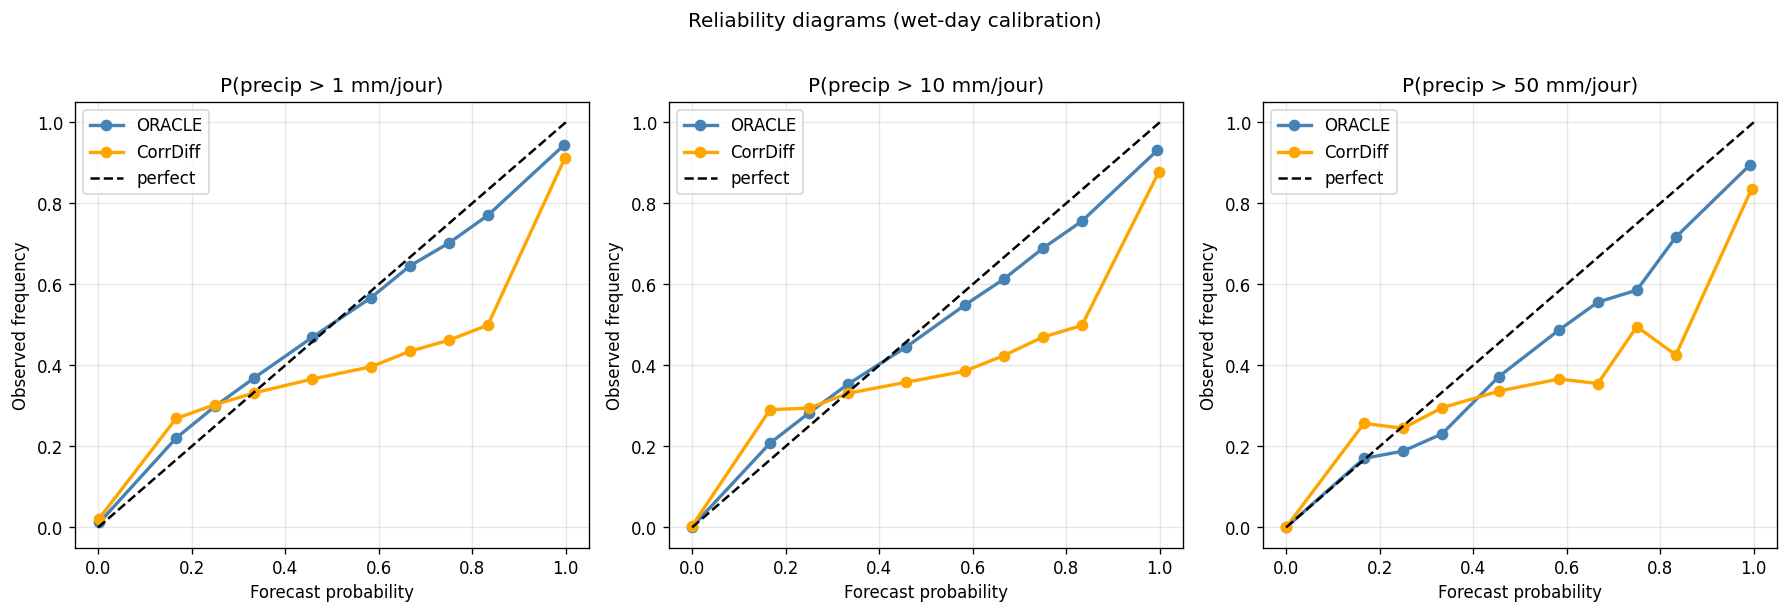
\includegraphics[width=0.80\linewidth]{../results/v5_evaluation/phase9_climate_standards/03_reliability.png}
  \par\vspace{0.15cm}
  {\small Diagrammes de fiabilité, $P(\mathrm{precip} > \{1, 10, 50\}$ mm/j$)$.
  \Oracle{} (bleu) suit la diagonale ; la baseline Noncausal (orange) reste
  sous-confiante aux probabilités élevées. Sous-dispersion résiduelle à $>50$ mm/j.}
\end{frame}

% 32 — EXTREMES
\begin{frame}{Extrêmes : biais réduits sur RX1day et R10mm, distance spectrale divisée par 450}
  \centering
  \small
  \begin{tabular}{l c c l}
    \toprule
    \textbf{Biais (proche de 0 = mieux)} & \Oracle{} & \textbf{Noncausal} & \textbf{Lecture} \\
    \midrule
    RX1day (mm)      & \tgood{$-2{,}73$} & $-4{,}09$ & sous-prédiction réduite de 33\,\% \\
    R10mm (jours)    & \tgood{$+0{,}88$} & $+2{,}65$ & gain $-67\,\%$ \\
    CDD (jours)      & $+17{,}95$ & $+21{,}51$ & \tbad{surestimé des deux côtés} \\
    Distance PSD     & \tgood{0,001} & 0,447 & $\div 450$ \\
    \bottomrule
  \end{tabular}
  \par\vspace{0.25cm}
  \begin{itemize}
    \item La baseline lissait les échelles 30--80 km ; \Oracle{} devient \emph{skillful}
          (FSS) dès $\sim$30 km contre $\sim$80 km, et restitue la queue droite là où
          \CorrDiff{} tronque au-delà de $\sim$30 mm/j.
    \item CDD : biais hérité de la perte MSE --- aucune valeur opérationnelle revendiquée
          pour la sécheresse.
  \end{itemize}
\end{frame}

% 33 — RETURN PERIOD
\begin{frame}{Périodes de retour : \Oracle{} suit la vérité là où la baseline sature}
  \centering
  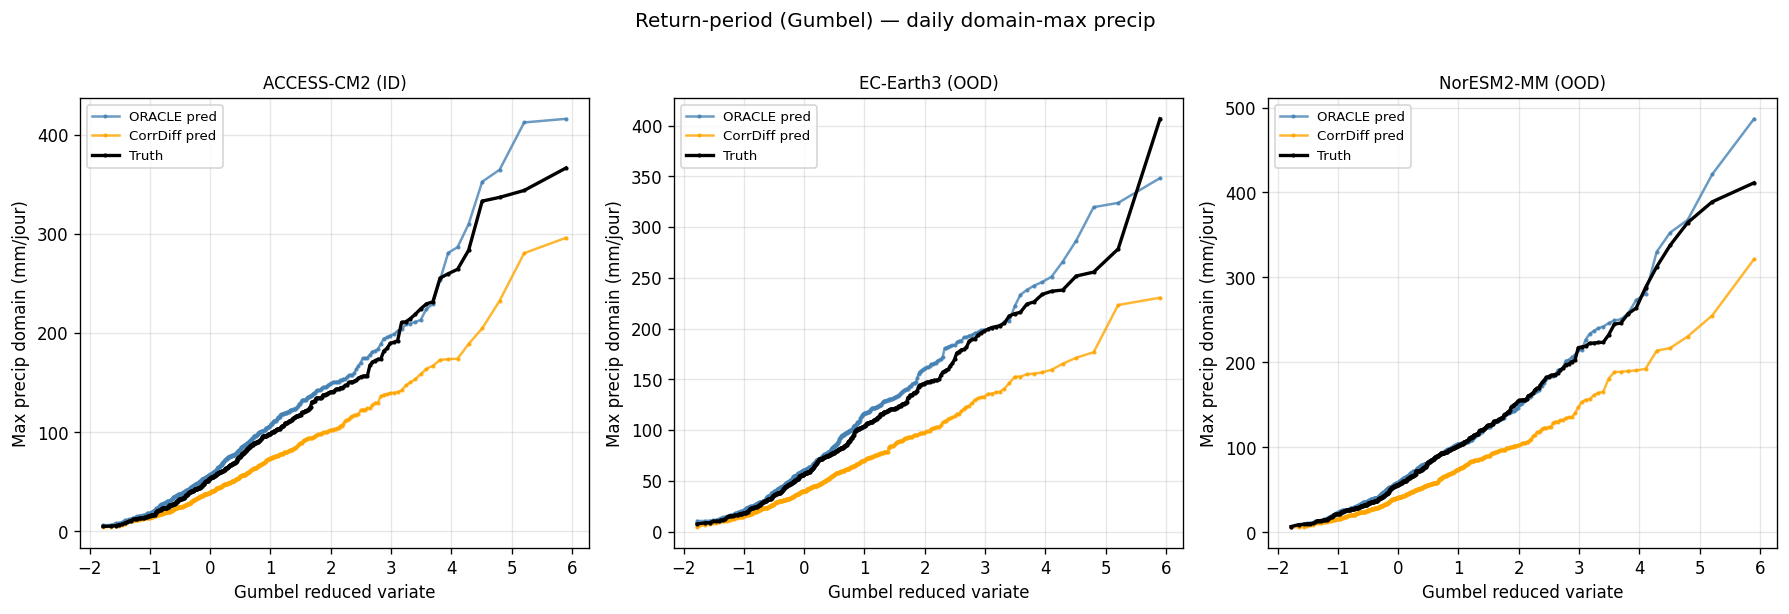
\includegraphics[width=0.80\linewidth]{../results/v5_evaluation/phase9_climate_standards/02_return_period.png}
  \par\vspace{0.15cm}
  {\small Courbes de Gumbel, précipitation journalière maximale --- en distribution
  (ACCESS-CM2) \emph{et} sur les deux GCM jamais vus. \Oracle{} (bleu) suit la vérité
  (noir) jusqu'aux périodes les plus longues ; la baseline Noncausal (orange) sature
  systématiquement sous les extrêmes observés.}
\end{frame}

% 34 — INTER-GCM
\begin{frame}{Robustesse inter-GCM : le gain persiste sur deux modèles jamais vus}
  \centering
  \small
  \begin{tabular}{l cc cc c}
    \toprule
    & \multicolumn{2}{c}{\Oracle{}} & \multicolumn{2}{c}{\textbf{Noncausal}} & \\
    \cmidrule(lr){2-3}\cmidrule(lr){4-5}
    \textbf{GCM} & CRPS & spr/RMSE & CRPS & spr/RMSE & $\Delta$ CRPS \\
    \midrule
    ACCESS-CM2 (réf.\ ID)   & 0,249 & 0,686 & 0,415 & 0,197 & \tgood{$-40\,\%$} \\
    EC-Earth3 (inter-GCM)   & 0,319 & 0,575 & 0,457 & 0,183 & \tgood{$-30\,\%$} \\
    NorESM2-MM (inter-GCM)  & 0,342 & 0,593 & 0,478 & 0,196 & \tgood{$-28\,\%$} \\
    \bottomrule
  \end{tabular}
  \par\vspace{0.25cm}
  \begin{itemize}
    \item \Oracle{} reste $1{,}4\times$ meilleur en valeur absolue sur des GCM
          \emph{jamais vus à l'entraînement}, avec un spread-skill $3\times$ supérieur.
    \item Lecture honnête : le gain causal porte sur le \emph{niveau} d'erreur, pas sur
          la \emph{pente} de dégradation --- et le régime reste historique
          (le test SSP futur est en perspective).
  \end{itemize}
\end{frame}

% 35 — INTERVENTIONS
\begin{frame}{Perturbations contrôlées : \Oracle{} répond avec le bon signe, deux fois sur deux}
  \centering
  \small
  \begin{tabular}{l l c c}
    \toprule
    \textbf{Modèle} & \textbf{Perturbation} & $\delta_{\mathrm{moy}}$ ($\times 10^{-3}$) & \textbf{Signe attendu ?} \\
    \midrule
    \Oracle{}  & $q_{850} + 20\,\%$        & $+1{,}24$ & \tgood{oui} (cohérent Clausius--Clapeyron) \\
    \Oracle{}  & $t_{850} + 3\,\mathrm{K}$ & $+0{,}84$ & \tgood{oui} (cohérent Clausius--Clapeyron) \\
    Noncausal  & $q_{850} + 20\,\%$        & $+0{,}55$ & oui \\
    Noncausal  & $t_{850} + 3\,\mathrm{K}$ & $-0{,}84$ & \tbad{\textbf{non}} (signe inversé) \\
    \bottomrule
  \end{tabular}
  \par\vspace{0.05cm}
  {\scriptsize IC bootstrap 95\,\% excluant 0 dans les quatre cas ; $n=30$ jours par perturbation.}
  \vspace{0.2cm}
  \begin{block}{Pourquoi la baseline échoue sur la température}
    \small Elle a appris la corrélation observationnelle « température élevée
    $\leftrightarrow$ régimes anticycloniques secs » de la Nouvelle-Zélande, au lieu de
    la relation thermodynamique qui agirait \emph{toutes choses égales par ailleurs}.
  \end{block}
\end{frame}

% 36 — INTEGRATED GRADIENTS
\begin{frame}{Le modèle causal exploite réellement ses variables d'entrée}
  \centering
  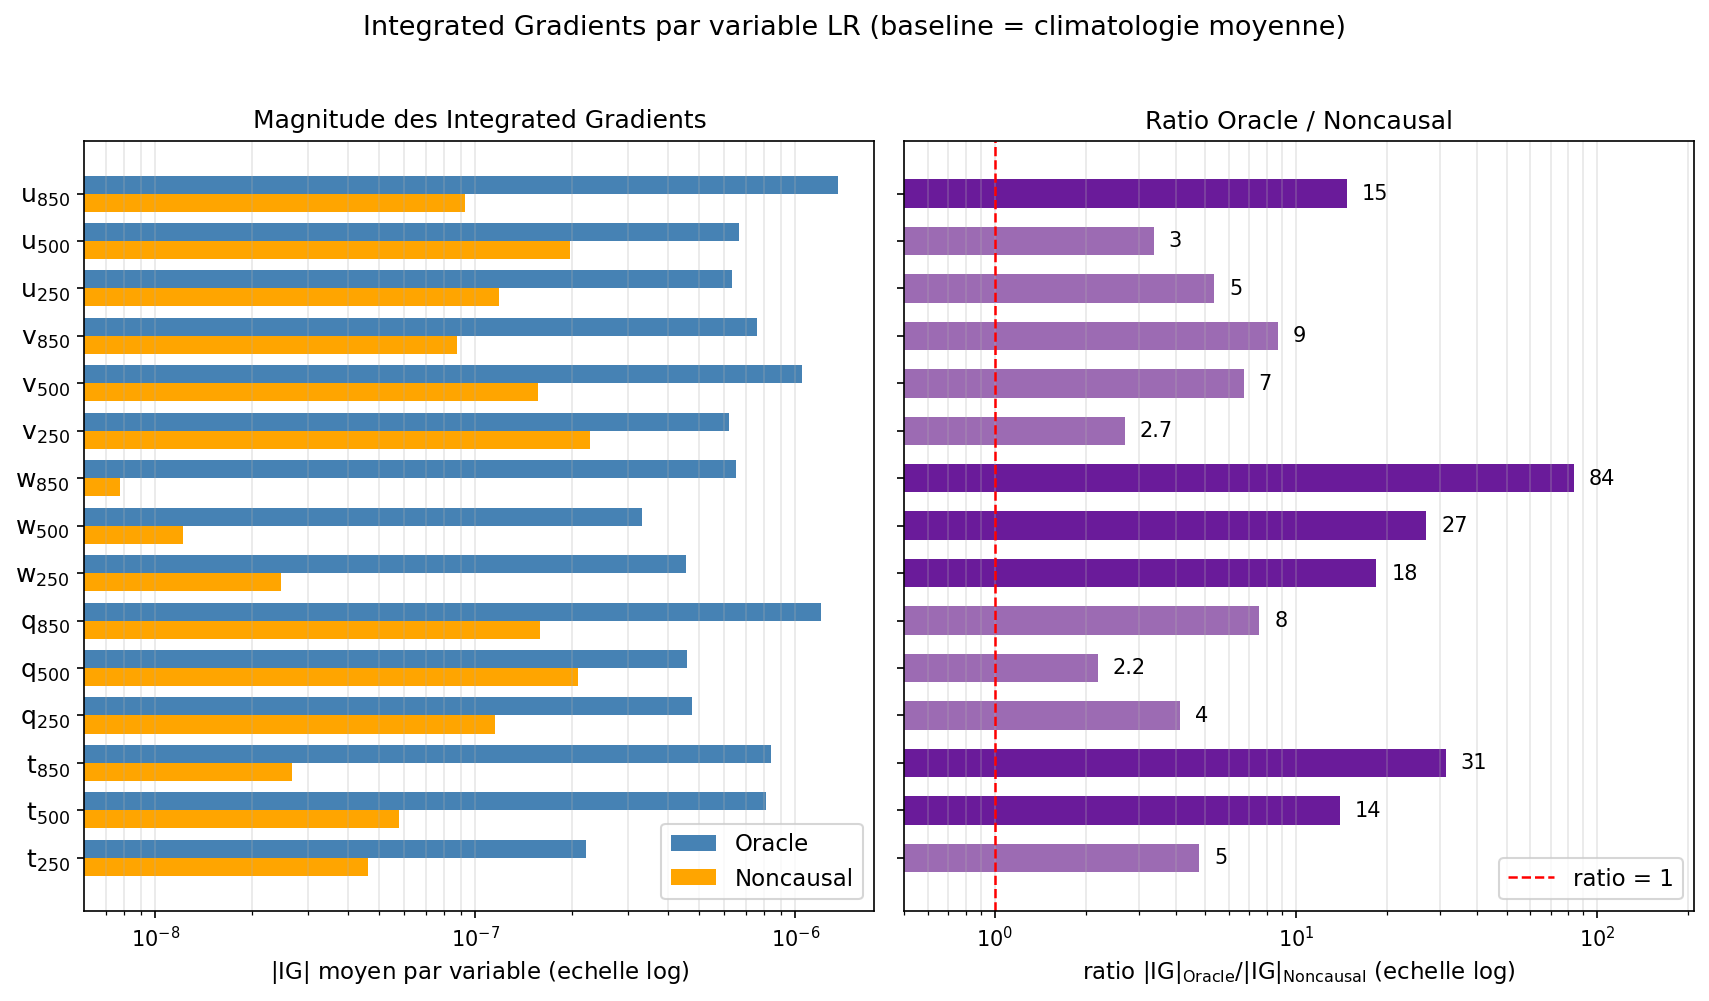
\includegraphics[width=0.78\linewidth]{../results/v5_evaluation/phase12_integrated_gradients/01_integrated_gradients.png}
  \par\vspace{0.15cm}
  {\small Integrated Gradients agrégés par variable LR. \textbf{Gauche} : \Oracle{} (bleu)
  exploite chaque variable un à deux ordres de grandeur de plus que la baseline
  Noncausal (orange). \textbf{Droite} : les leviers dominants sont physiquement sensés ---
  vitesse verticale ($w_{850}$, $w_{500}$) et température ($t_{850}$).}
\end{frame}

% 37 — CE QUE LE DAG APPREND
\begin{frame}{Ce que le DAG apprend --- et ce qu'il n'apprend pas}
  \begin{columns}[T]
    \begin{column}{0.48\textwidth}
      \textbf{À 6 n\oe{}uds (configuration principale)}
      \small
      \begin{itemize}
        \item Magnitudes \tbad{plates} ($\approx 0{,}18$ partout), $Q_{\mathrm{phys}} = 0{,}40$.
        \item Limite d'identifiabilité \emph{observationnelle} d'un SCM (Pearl) :
              le DAG appris est une \emph{régularisation topologique}, pas une
              cartographie causale identifiée.
      \end{itemize}
    \end{column}
    \begin{column}{0.48\textwidth}
      \textbf{À 9 n\oe{}uds (un n\oe{}ud par variable)}
      \small
      \begin{itemize}
        \item $Q_{\mathrm{phys}}^{\mathrm{continu}} = \tgood{0{,}9997}$,
              squelette $F1 = \tgood{1{,}0}$, zéro arête parasite.
        \item La platitude n'est \alert{pas un plafond architectural} : c'est le prix
              de l'agrégation choisie pour la lisibilité humaine.
      \end{itemize}
    \end{column}
  \end{columns}
  \vspace{0.25cm}
  \begin{block}{L'asymétrie à retenir ($Q_{\mathrm{int}} = 2/2$ vs $Q_{\mathrm{phys}} = 0{,}40$)}
    \small Signes interventionnels corrects \emph{sans} magnitudes identifiées :
    le DAG rend le modèle \textbf{intervenable} et \textbf{vérifiable} (O3) ---
    c'est son rôle, distinct de celui du gain de skill.
  \end{block}
\end{frame}

% =====================================================================
\section{Discussion et conclusion}
% =====================================================================

% 38 — LIMITES
\begin{frame}{Cinq limites assumées}
  \begin{enumerate}
    \item \textbf{Magnitudes interventionnelles} $\approx$ trois ordres de grandeur sous
          Clausius--Clapeyron ($0{,}01\,\%/\mathrm{K}$ vs $\sim 7\,\%/\mathrm{K}$) :
          le signe est correct, la magnitude non --- contrôle de cohérence, \alert{pas
          outil de projection}.
    \item \textbf{Inter-GCM historique} $\neq$ vrai test hors-distribution climatique
          (validation SSP5-8.5 en perspective immédiate).
    \item \textbf{Aucune donnée africaine testée} ; la métrique F1@p99 régresse
          ($-6{,}9\,\%$, régularisation lissante interne).
    \item \textbf{Un seul seed} d'entraînement (contrainte de calcul) ; ensembles modestes
          ($K = 12$/$64$ contre 192 chez \CorrDiff{}).
    \item \textbf{Orographie HR absente en entrée} : le déficit RX1day se concentre sur
          le versant ouest des Alpes du Sud --- limite \emph{isolable}, partagée par
          toutes les baselines du domaine.
  \end{enumerate}
\end{frame}

% 39 — PERSPECTIVES
\begin{frame}{Perspectives : trois horizons, cap sur l'Afrique}
  \begin{description}
    \item[Court terme (1--2 mois)] Recalibration d'ensemble post-hoc (EMOS/BMA) ;
      validation sur \alert{SSP5-8.5} --- transforme le test inter-GCM historique en
      véritable test hors-distribution, sans modification architecturale.
    \item[Moyen terme (3--6 mois)] Ancrage prédictif joint type CASTLE (chaque arête de
      $\Adag$ forcée à porter un signal) ; masque physique
      $\lambda_{\mathrm{prior}} \|\Adag - \alpha G_{\mathrm{phys}}\|^2$.
    \item[Long terme (1--3 ans)] \textbf{Transfert africain} : sanity-check zéro-shot
      (Hautes Terres éthiopiennes, Sahel ouest, cible CHIRPS), puis ré-entraînement sur
      prédicteurs adaptés (mousson, ondes d'Est, ITCZ) et \alert{prior causal révisé} ---
      convection profonde ascendante, là où le prior néo-zélandais encode un couplage
      descendant.
  \end{description}
\end{frame}

% 40 — CONCLUSION
\begin{frame}{Conclusion : la causalité utile est une contrainte architecturale}
  \small
  \begin{enumerate}
    \item[\textbf{C1}] Une architecture two-stage où la causalité est inscrite dans la
      \textbf{topologie du chemin de calcul} --- indéfaisable par construction.
    \item[\textbf{C2}] Le \textbf{réseau causal récurrent} : SCM dynamique $+$ GRU $+$
      DAGMA dans une seule cellule.
    \item[\textbf{C3}] Une \textbf{interface inter-étages} par concaténation garantissant
      qu'aucune information ne contourne le chemin causal (O3 $= 0{,}87$).
    \item[\textbf{C4}] Un \textbf{protocole} à six familles de métriques avec deux
      diagnostics causaux originaux (ratio O3, $Q_{\mathrm{int}}$).
  \end{enumerate}
  \vspace{0.15cm}
  \centering
  CRPS \tgood{$-40\,\%$} ID \quad CRPS \tgood{$-30\,\%$} inter-GCM \quad
  spread-skill \tgood{$\times 3{,}5$} \quad $Q_{\mathrm{int}}$ \tgood{2/2} vs 1/2
  \vspace{0.2cm}
  \begin{block}{}
    \centering\small\itshape La causalité utile au downscaling n'est pas une propriété
    décorative émergeant d'une régularisation, mais une contrainte à placer explicitement
    dans le graphe de calcul. Elle fait ses preuves en Nouvelle-Zélande aujourd'hui ;
    elle devra les refaire demain dans les communautés d'Afrique centrale qui ont motivé
    ce travail.
  \end{block}
\end{frame}

% 41 — MERCI
\begin{frame}[plain]
  \vfill
  \centering
  {\Huge\bfseries\color{uridarkblue} Merci de votre attention}\\[0.6cm]
  {\large Questions ?}\\[1.0cm]
  {\footnotesize KENFACK Leonel --- Université de Dschang, URIFIA\\
  Sous la direction du Pr.~BOMGNI Alain Bertrand}
  \vfill
\end{frame}

% =====================================================================
% BACKUPS (pour les questions du jury)
% =====================================================================
\section*{Annexes}

\begin{frame}{Backup A --- Métriques ponctuelles en distribution (espace $\log(1+p)$)}
  \centering
  \small
  \begin{tabular}{l c c c}
    \toprule
    \textbf{Métrique} & \Oracle{} & \textbf{Noncausal} & $\Delta_{\mathrm{rel}}$ \\
    \midrule
    RMSE               & 0,124 & 0,130 & $-4{,}1\,\%$ \\
    MAE                & 0,060 & 0,064 & $-5{,}7\,\%$ \\
    Pearson global     & 0,825 & 0,819 & $+0{,}7\,\%$ (n.s.) \\
    F1@p95             & 0,650 & 0,656 & $-0{,}8\,\%$ \\
    F1@p99             & 0,512 & 0,550 & \tbad{$-6{,}9\,\%$} \\
    RAPSD distance     & 241,8 & 270,1 & $-10{,}5\,\%$ \\
    \bottomrule
  \end{tabular}
  \par\vspace{0.25cm}
  {\small Ensemble $K=64$, IC bootstrap 95\,\%. Nous ne défendons pas \Oracle{} comme
  Pareto-dominant sur RMSE/F1@p99 pooled, mais comme la première version dont l'apport
  causal architectural est \emph{mesurable}. La régression F1@p99 est analysée en annexe
  du mémoire (régularisation lissante).}
\end{frame}

\begin{frame}{Backup B --- Cartes de réponse aux interventions}
  \centering
  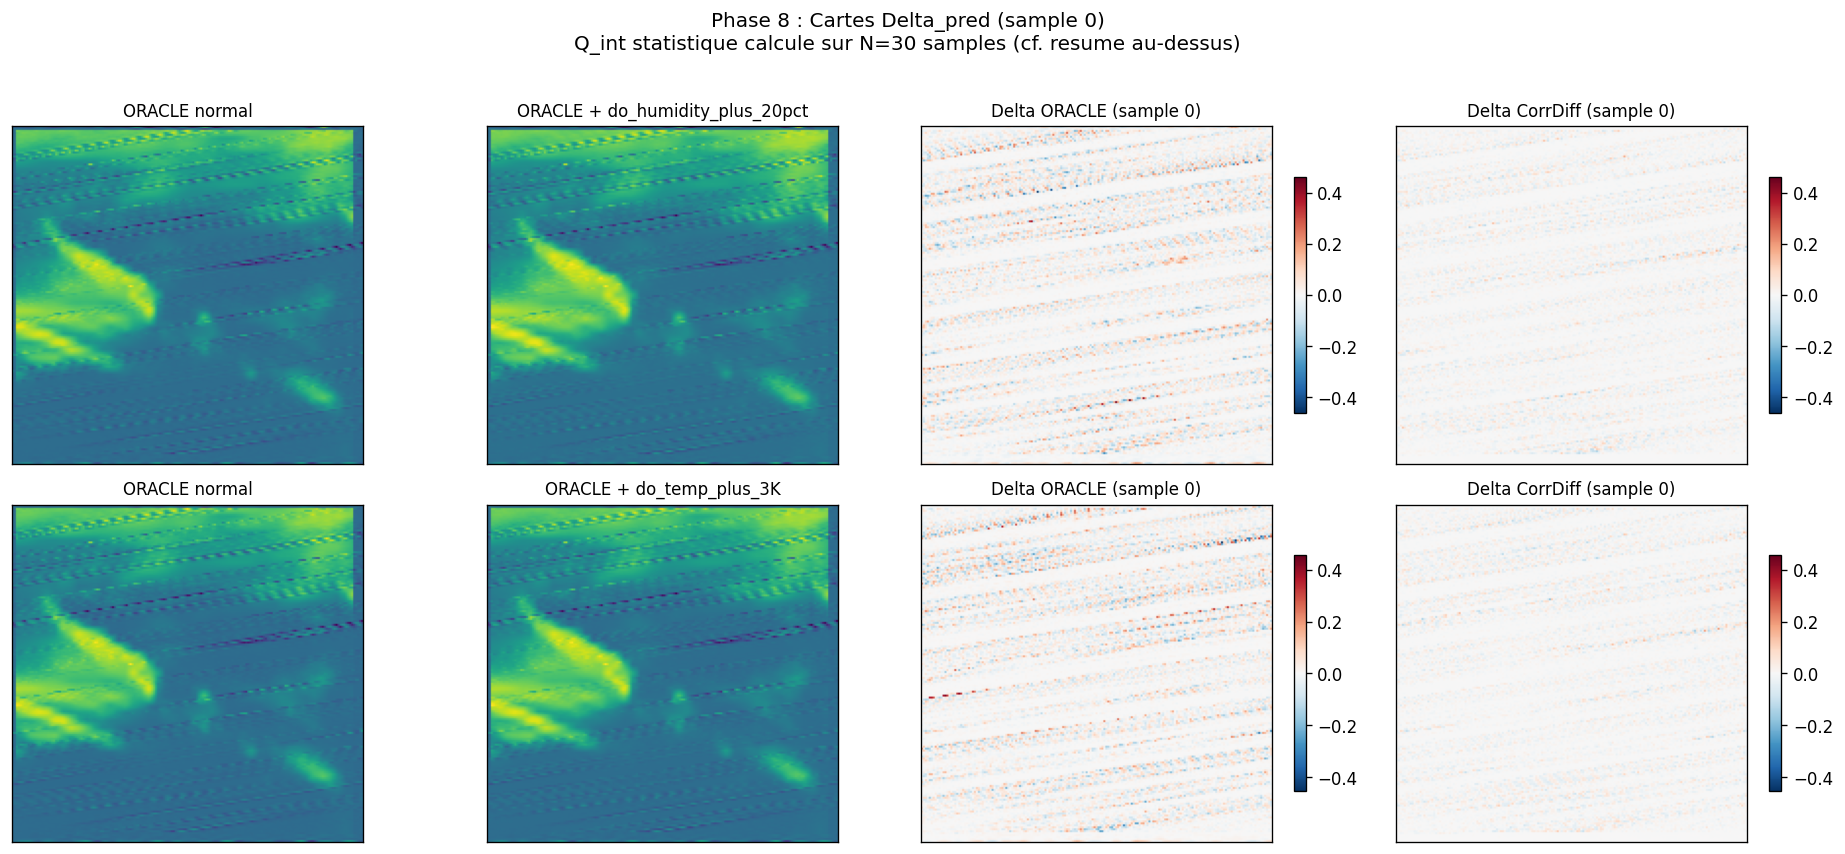
\includegraphics[width=0.70\linewidth]{../results/v5_evaluation/phase8_figures/03_interventions_maps.png}
  \par\vspace{0.1cm}
  {\small Réponse spatiale aux perturbations contrôlées (annexe IV du mémoire) :
  la réponse d'\Oracle{} est distribuée et du bon signe ; magnitudes en $10^{-3}$
  unités relatives.}
\end{frame}

\begin{frame}{Backup C --- Où se concentre le biais d'extrêmes ?}
  \centering
  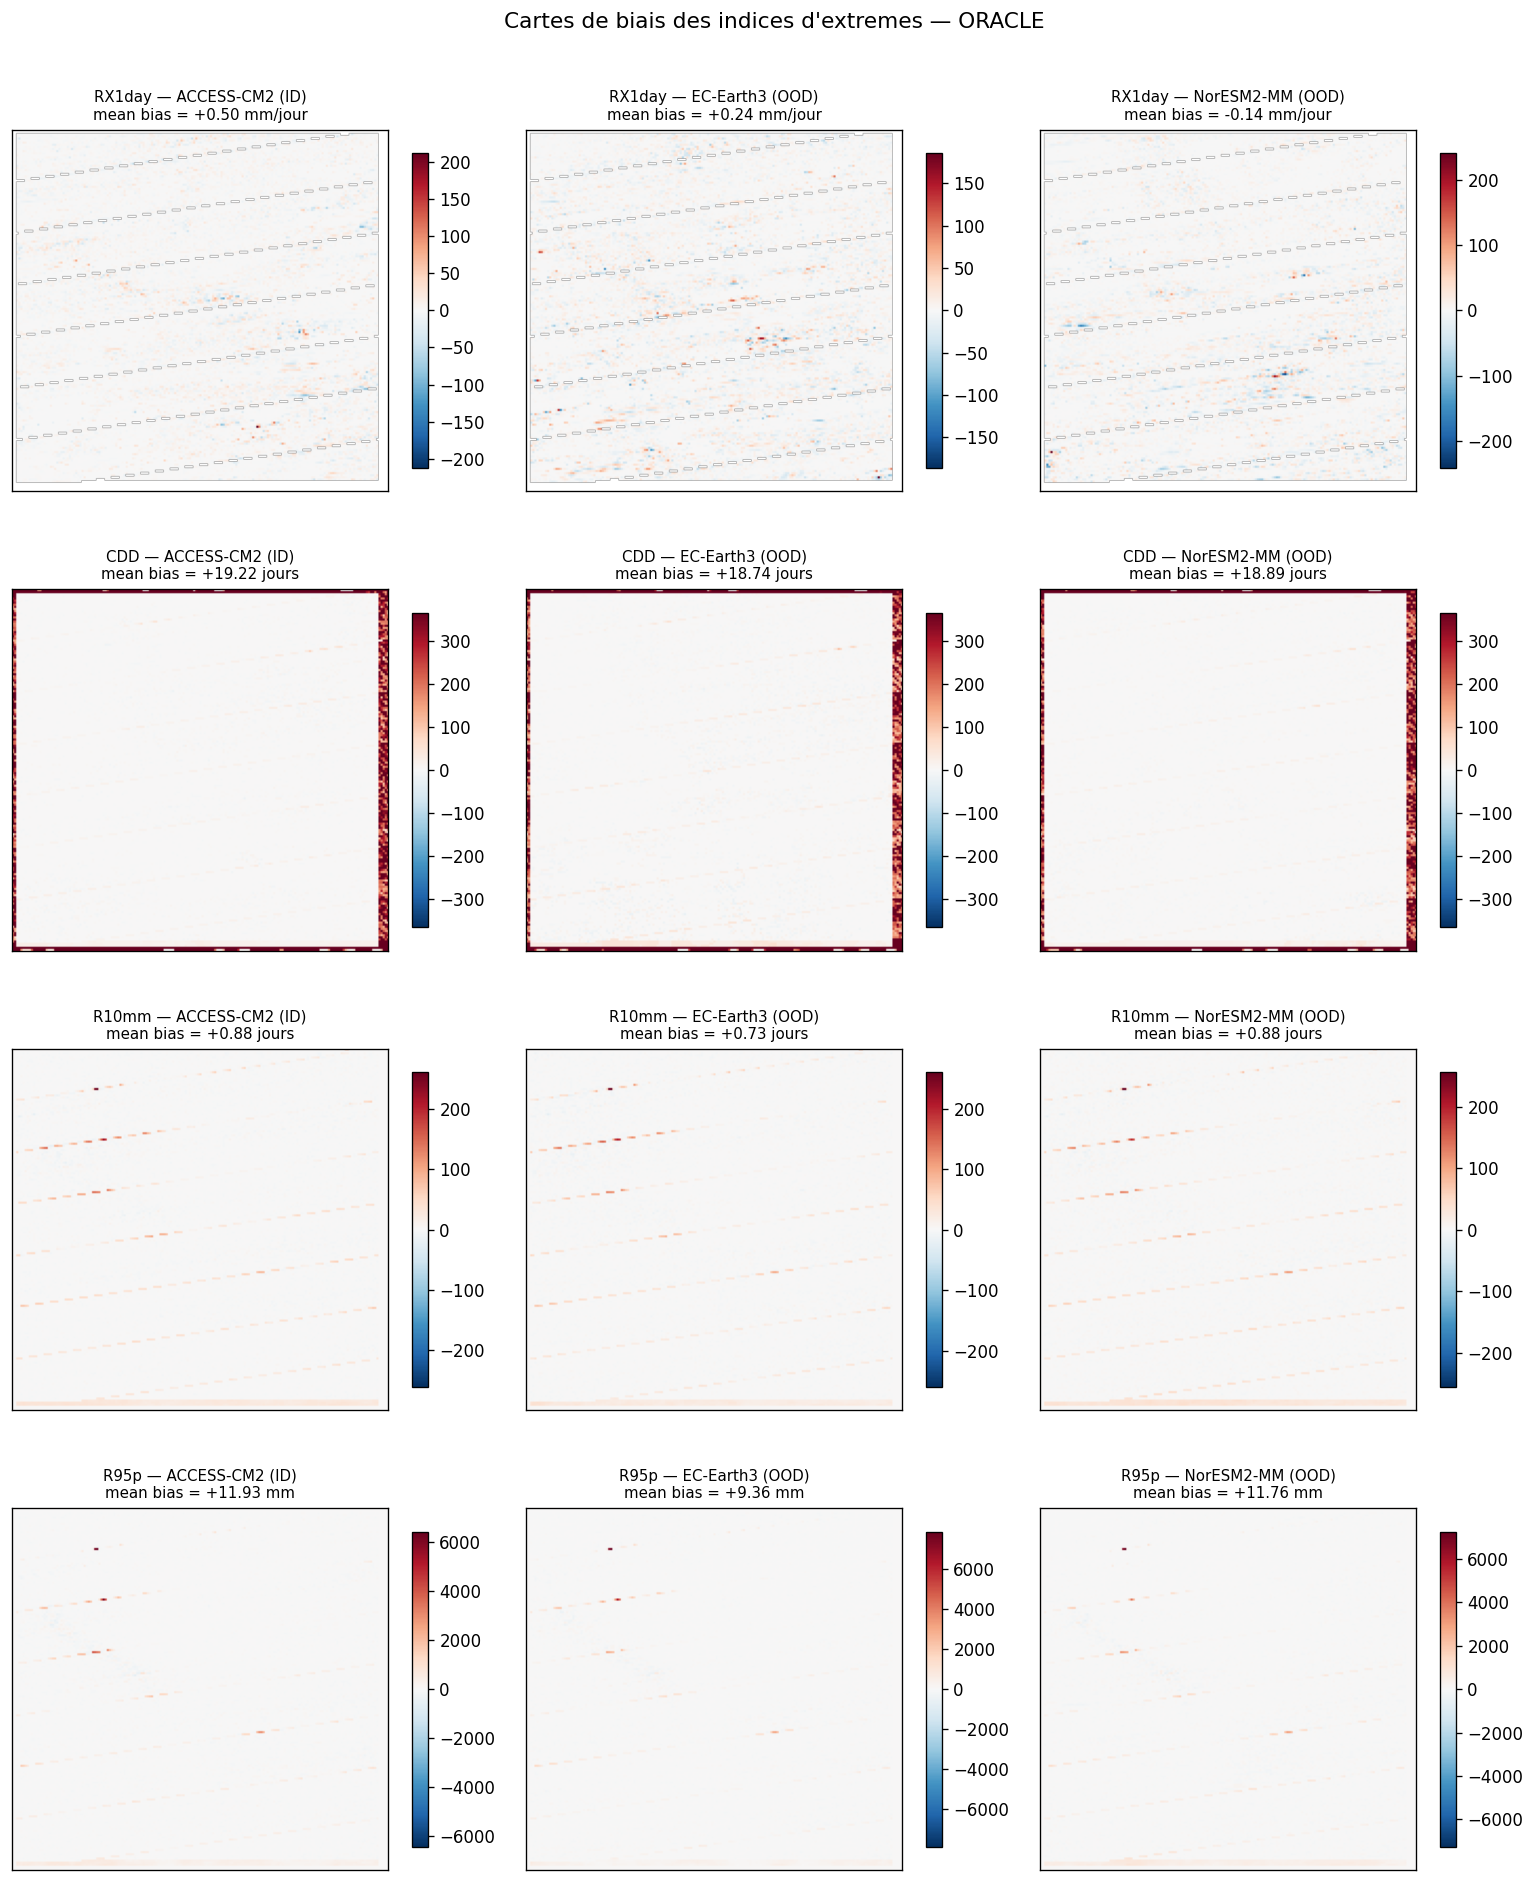
\includegraphics[height=0.62\textheight, keepaspectratio]{../results/v5_evaluation/phase10_extreme_bias_maps/extreme_bias_ORACLE.png}
  \par\vspace{0.1cm}
  {\small Biais RX1day d'\Oracle{} concentré sur le versant occidental des Alpes du Sud
  (annexe IV du mémoire) : signature de l'\alert{absence de DEM haute résolution en
  entrée}, partagée par \CorrDiff{} et le cGAN néo-zélandais --- limite isolable,
  première piste corrective.}
\end{frame}

\end{document}
